\documentclass[tikz,border=12pt]{standalone}
% Shared visual language for standalone EMT block diagrams.
\usepackage{amsmath}
\usetikzlibrary{arrows.meta,backgrounds,calc,fit,positioning}

\tikzset{
    emt diagram/.style = {>={Stealth[length=2.4mm]}},
    line/.style        = {semithick, rounded corners=6pt},
    block/.style       = {draw, semithick, fill=white,
                          minimum height=1cm, minimum width=2.3cm},
    hblock/.style      = {block, minimum width=2.24cm, minimum height=1.3cm},
    vblock/.style      = {block, minimum width=1.3cm, minimum height=2.24cm},
    sum/.style         = {draw, semithick, fill=white, circle,
                          inner sep=2.6pt},
    signal/.style      = {circle, fill, inner sep=1.4pt,
                          label distance=3pt},
    sig/.style         = {font=\small},
    pm/.style          = {font=\scriptsize},
    wire jump/.style   = {line,
                          preaction={draw=white, line width=3pt,
                                     line cap=round}},
    enclosure/.style   = {draw, dashed, semithick, rounded corners=4pt},
    operator enclosure/.style = {enclosure, inner xsep=7mm, inner ysep=6mm}
}


% TUNABLES: gain width and separation of the three control panels.
\def\gainwidth{1.35cm}
\def\qrow{-10.1}
\def\terminalrow{-21.0}

\begin{document}
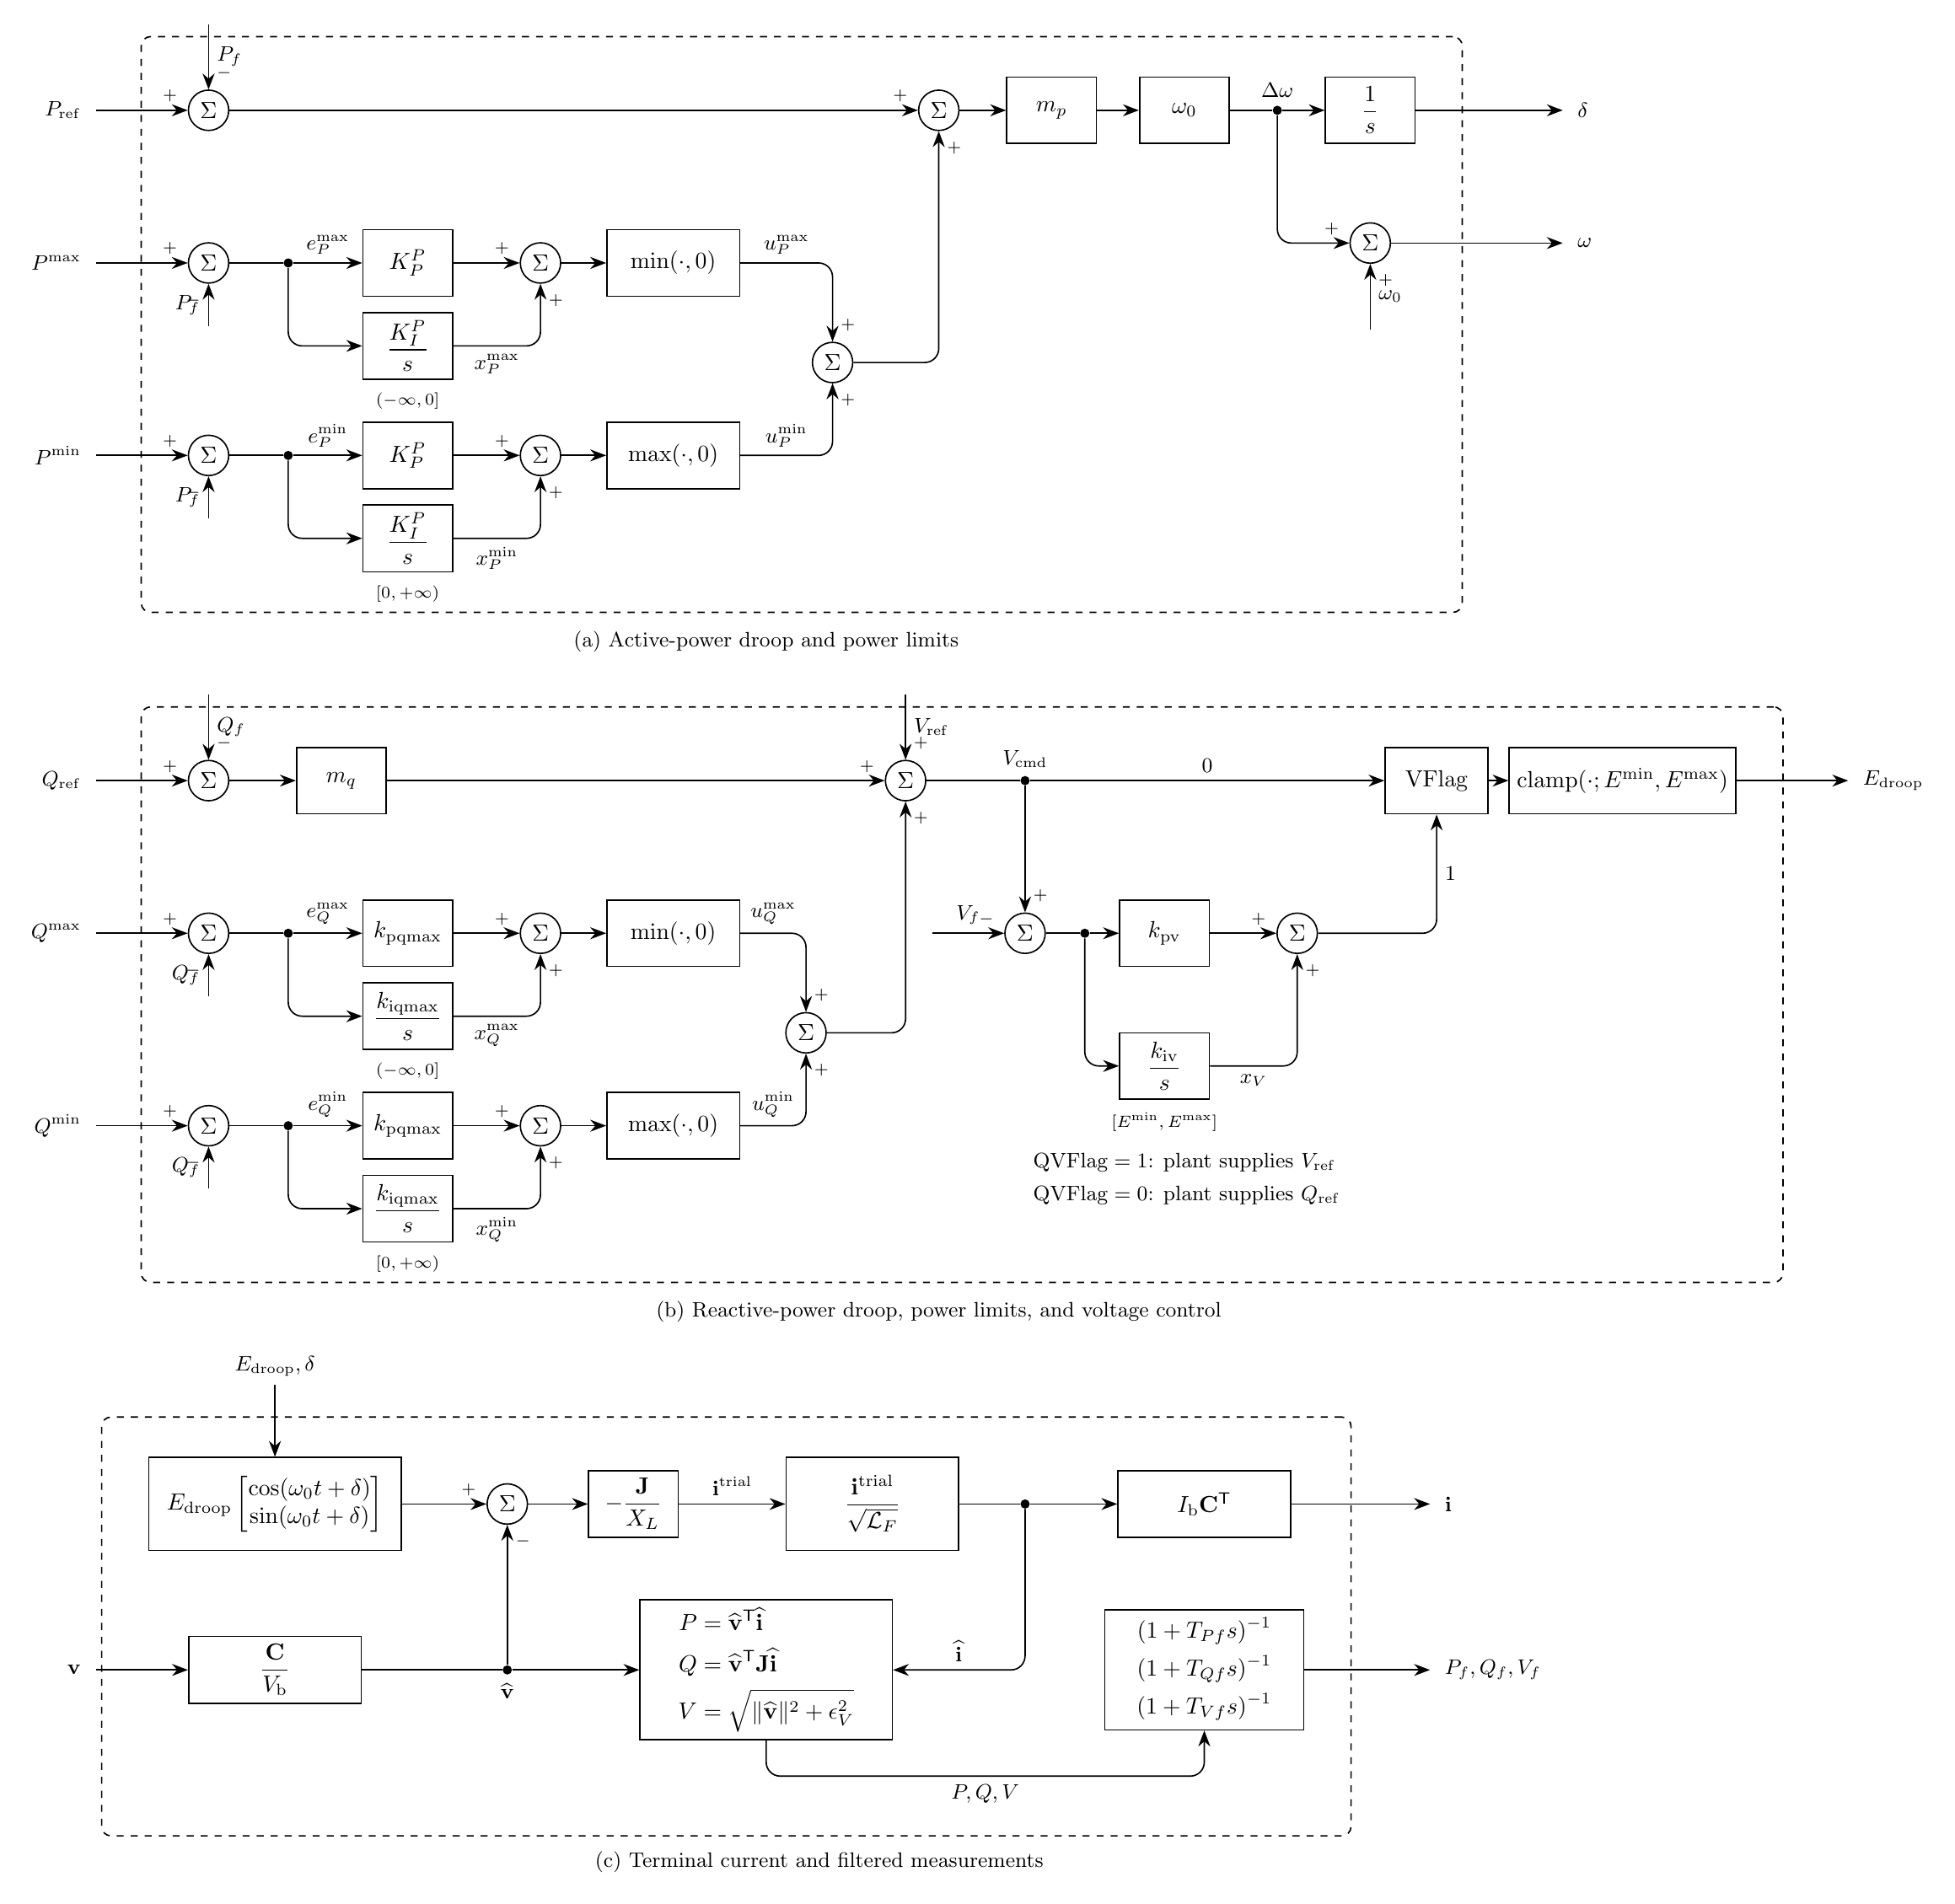
\begin{tikzpicture}[emt diagram]

% Active-power droop, with independent upper and lower limited PI paths.
\node[sum] (pe) at (0,0) {$\Sigma$};
\node[block, minimum width=\gainwidth] (mp) at (12.7,0) {$m_p$};
\node[sum] (dw) at (11,0) {$\Sigma$};
\node[block, minimum width=\gainwidth] (w0) at (14.7,0) {$\omega_0$};
\node[signal, label={[sig]above:$\Delta\omega$}] (dwsplit) at (16.1,0) {};
\node[block, minimum width=\gainwidth] (angle) at (17.5,0) {$\dfrac{1}{s}$};
\node[sig, anchor=east] at (-1.8,0) {$P_\mathrm{ref}$};
\draw[->, line] (-1.7,0) -- (pe.west);
\node[pm, above left=0pt and 1pt of pe.west] {$+$};
\draw[->, line] (0,1.3) -- node[sig, right] {$P_f$} (pe.north);
\node[pm, above right=1pt and 0pt of pe.north] {$-$};
\draw[->, line] (pe.east) -- (dw.west);
\node[pm, above left=0pt and 1pt of dw.west] {$+$};
\draw[->, line] (dw.east) -- (mp.west);
\draw[->, line] (mp.east) -- (w0.west);
\draw[line] (w0.east) -- (dwsplit);
\draw[->, line] (dwsplit) -- (angle.west);
\draw[->, line] (angle.east) -- (20.4,0);
\node[sig, anchor=west] at (20.5,0) {$\delta$};
\node[sum] (omega) at (17.5,-2.0) {$\Sigma$};
\draw[->, line] (dwsplit) |- (omega.west);
\node[pm, above left=0pt and 1pt of omega.west] {$+$};
\draw[->, line] (17.5,-3.3) -- node[sig, right] {$\omega_0$} (omega.south);
\node[pm, below right=1pt and 0pt of omega.south] {$+$};
\draw[->, line] (omega.east) -- (20.4,-2.0);
\node[sig, anchor=west] at (20.5,-2.0) {$\omega$};

\foreach \name/\yy/\bound/\limit/\interval in {
    pmax/-2.3/\max/\min/{(-\infty,0]},
    pmin/-5.2/\min/\max/{[0,+\infty)}} {
    \node[sum] (\name-error) at (0,\yy) {$\Sigma$};
    \node[signal] (\name-split) at (1.2,\yy) {};
    \node[block, minimum width=\gainwidth] (\name-kp)
        at (3,\yy) {$K_P^P$};
    \node[block, minimum width=\gainwidth] (\name-integral)
        at (3,\yy-1.25) {$\dfrac{K_I^P}{s}$};
    \node[pm, below=2pt of \name-integral] {$\interval$};
    \node[sum] (\name-sum) at (5,\yy) {$\Sigma$};
    \node[block, minimum width=2.0cm] (\name-limit)
        at (7,\yy) {$\limit(\cdot,0)$};
    \node[sig, anchor=east] at (-1.8,\yy) {$P^{\bound}$};
    \draw[->, line] (-1.7,\yy) -- (\name-error.west);
    \node[pm, above left=0pt and 1pt of \name-error.west] {$+$};
    \draw[->, line] (0,\yy-.95) -- node[sig, left] {$P_f$} (\name-error.south);
    \node[pm, below left=1pt and 0pt of \name-error.south] {$-$};
    \draw[line] (\name-error.east) -- (\name-split);
    \draw[->, line] (\name-split) -- node[sig, above] {$e_P^{\bound}$} (\name-kp.west);
    \draw[->, line] (\name-split) |- (\name-integral.west);
    \draw[->, line] (\name-kp.east) -- (\name-sum.west);
    \node[pm, above left=0pt and 1pt of \name-sum.west] {$+$};
    \draw[->, line] (\name-integral.east) -| node[sig, near start, below]
        {$x_P^{\bound}$} (\name-sum.south);
    \node[pm, below right=1pt and 0pt of \name-sum.south] {$+$};
    \draw[->, line] (\name-sum.east) -- (\name-limit.west);
}
\node[sum] (plimits) at (9.4,-3.8) {$\Sigma$};
\draw[->, line] (pmax-limit.east) -| node[sig, near start, above]
    {$u_P^{\max}$} (plimits.north);
\node[pm, above right=1pt and 0pt of plimits.north] {$+$};
\draw[->, line] (pmin-limit.east) -| node[sig, near start, above]
    {$u_P^{\min}$} (plimits.south);
\node[pm, below right=1pt and 0pt of plimits.south] {$+$};
\draw[->, line] (plimits.east) -| (dw.south);
\node[pm, below right=1pt and 0pt of dw.south] {$+$};
\node[sig] at (8.4,-8.0) {(a) Active-power droop and power limits};
\begin{scope}[on background layer]
    \node[operator enclosure,
        fit=(pe)(mp)(dw)(w0)(angle)(omega)(plimits)
            (pmax-error)(pmin-error)(pmin-integral)(pmin-limit)] {};
\end{scope}

% Reactive-power droop and limits use the same one-sided PI structure.
\begin{scope}[yshift=\qrow cm]
\node[sum] (qe) at (0,0) {$\Sigma$};
\node[block, minimum width=\gainwidth] (mq) at (2,0) {$m_q$};
\node[sum] (vcmd) at (10.5,0) {$\Sigma$};
\node[sig, anchor=east] at (-1.8,0) {$Q_\mathrm{ref}$};
\draw[->, line] (-1.7,0) -- (qe.west);
\node[pm, above left=0pt and 1pt of qe.west] {$+$};
\draw[->, line] (0,1.3) -- node[sig, right] {$Q_f$} (qe.north);
\node[pm, above right=1pt and 0pt of qe.north] {$-$};
\draw[->, line] (qe.east) -- (mq.west);
\draw[->, line] (mq.east) -- (vcmd.west);
\node[pm, above left=0pt and 1pt of vcmd.west] {$+$};
\draw[->, line] (10.5,1.3) -- node[sig, right] {$V_\mathrm{ref}$} (vcmd.north);
\node[pm, above right=1pt and 0pt of vcmd.north] {$+$};
\foreach \name/\yy/\bound/\limit/\interval in {
    qmax/-2.3/\max/\min/{(-\infty,0]},
    qmin/-5.2/\min/\max/{[0,+\infty)}} {
    \node[sum] (\name-error) at (0,\yy) {$\Sigma$};
    \node[signal] (\name-split) at (1.2,\yy) {};
    \node[block, minimum width=\gainwidth] (\name-kp)
        at (3,\yy) {$k_{\mathrm{pqmax}}$};
    \node[block, minimum width=\gainwidth] (\name-integral)
        at (3,\yy-1.25) {$\dfrac{k_{\mathrm{iqmax}}}{s}$};
    \node[pm, below=2pt of \name-integral] {$\interval$};
    \node[sum] (\name-sum) at (5,\yy) {$\Sigma$};
    \node[block, minimum width=2.0cm] (\name-limit)
        at (7,\yy) {$\limit(\cdot,0)$};
    \node[sig, anchor=east] at (-1.8,\yy) {$Q^{\bound}$};
    \draw[->, line] (-1.7,\yy) -- (\name-error.west);
    \node[pm, above left=0pt and 1pt of \name-error.west] {$+$};
    \draw[->, line] (0,\yy-.95) -- node[sig, left] {$Q_f$} (\name-error.south);
    \node[pm, below left=1pt and 0pt of \name-error.south] {$-$};
    \draw[line] (\name-error.east) -- (\name-split);
    \draw[->, line] (\name-split) -- node[sig, above] {$e_Q^{\bound}$} (\name-kp.west);
    \draw[->, line] (\name-split) |- (\name-integral.west);
    \draw[->, line] (\name-kp.east) -- (\name-sum.west);
    \node[pm, above left=0pt and 1pt of \name-sum.west] {$+$};
    \draw[->, line] (\name-integral.east) -| node[sig, near start, below]
        {$x_Q^{\bound}$} (\name-sum.south);
    \node[pm, below right=1pt and 0pt of \name-sum.south] {$+$};
    \draw[->, line] (\name-sum.east) -- (\name-limit.west);
}
\node[sum] (qlimits) at (9,-3.8) {$\Sigma$};
\draw[->, line] (qmax-limit.east) -| node[sig, near start, above]
    {$u_Q^{\max}$} (qlimits.north);
\node[pm, above right=1pt and 0pt of qlimits.north] {$+$};
\draw[->, line] (qmin-limit.east) -| node[sig, near start, above]
    {$u_Q^{\min}$} (qlimits.south);
\node[pm, below right=1pt and 0pt of qlimits.south] {$+$};
\draw[->, line] (qlimits.east) -| (vcmd.south);
\node[pm, below right=1pt and 0pt of vcmd.south] {$+$};

% VFlag selects direct internal-voltage control or terminal-voltage PI control.
\node[signal, label={[sig]above:$V_\mathrm{cmd}$}] (vsplit) at (12.3,0) {};
\node[sum] (ve) at (12.3,-2.3) {$\Sigma$};
\node[block, minimum width=\gainwidth] (kpv) at (14.4,-2.3) {$k_{\mathrm{pv}}$};
\node[sum] (vsum) at (16.4,-2.3) {$\Sigma$};
\node[block, minimum width=\gainwidth] (kiv) at (14.4,-4.3) {$\dfrac{k_{\mathrm{iv}}}{s}$};
\node[pm, below=2pt of kiv] {$[E^{\min},E^{\max}]$};
\node[block, minimum width=1.55cm] (vflag) at (18.5,0) {$\mathrm{VFlag}$};
\node[block, minimum width=2.6cm] (elim) at (21.3,0)
    {$\mathrm{clamp}(\cdot;E^{\min},E^{\max})$};
\draw[line] (vcmd.east) -- (vsplit);
\draw[->, line] (vsplit) -- node[sig, above] {$0$} (vflag.west);
\draw[->, line] (vsplit) -- (ve.north);
\node[pm, above right=1pt and 0pt of ve.north] {$+$};
\draw[->, line] (10.9,-2.3) -- node[sig, above] {$V_f$} (ve.west);
\node[pm, above left=0pt and 1pt of ve.west] {$-$};
\node[signal] (vesplit) at (13.2,-2.3) {};
\draw[line] (ve.east) -- (vesplit);
\draw[->, line] (vesplit) -- (kpv.west);
\draw[->, line] (vesplit) |- (kiv.west);
\draw[->, line] (kpv.east) -- (vsum.west);
\node[pm, above left=0pt and 1pt of vsum.west] {$+$};
\draw[->, line] (kiv.east) -| node[sig, near start, below] {$x_V$} (vsum.south);
\node[pm, below right=1pt and 0pt of vsum.south] {$+$};
\draw[->, line] (vsum.east) -| node[sig, near end, right] {$1$} (vflag.south);
\draw[->, line] (vflag.east) -- (elim.west);
\draw[->, line] (elim.east) -- (24.7,0);
\node[sig, anchor=west] at (24.8,0) {$E_\mathrm{droop}$};
\node[sig, align=left, anchor=west] at (12.3,-6.0)
    {$\mathrm{QVFlag}=1$: plant supplies $V_\mathrm{ref}$\\[3pt]
     $\mathrm{QVFlag}=0$: plant supplies $Q_\mathrm{ref}$};
\node[sig] at (11,-8.0) {(b) Reactive-power droop, power limits, and voltage control};
\begin{scope}[on background layer]
    \node[operator enclosure,
        fit=(qe)(mq)(vcmd)(qlimits)(qmax-error)(qmin-error)(qmin-integral)
            (ve)(kpv)(vsum)(kiv)(vflag)(elim)] {};
\end{scope}
\end{scope}

% Algebraic voltage source, direction-preserving fault limit, and measurements.
\begin{scope}[yshift=\terminalrow cm]
\node[block, minimum width=3.8cm, minimum height=1.4cm] (edroop) at (1,0)
    {$E_\mathrm{droop}\begin{bmatrix}
        \cos(\omega_0 t+\delta)\\\sin(\omega_0 t+\delta)
      \end{bmatrix}$};
\node[sum] (voltage) at (4.5,0) {$\Sigma$};
\node[block, minimum width=\gainwidth] (reactance) at (6.4,0) {$-\dfrac{\mathbf{J}}{X_L}$};
\node[block, minimum width=2.6cm, minimum height=1.4cm] (flimit) at (10,0)
    {$\dfrac{\mathbf{i}^{\mathrm{trial}}}{\sqrt{\mathcal{L}_F}}$};
\node[signal] (ic) at (12.3,0) {};
\node[block, minimum width=2.6cm] (abc) at (15,0) {$I_\mathrm{b}\mathbf{C}^{\mathsf{T}}$};
\node[sig, above] at (1,1.8) {$E_\mathrm{droop},\delta$};
\draw[->, line] (1,1.8) -- (edroop.north);
\draw[->, line] (edroop.east) -- (voltage.west);
\node[pm, above left=0pt and 1pt of voltage.west] {$+$};
\draw[->, line] (voltage.east) -- (reactance.west);
\draw[->, line] (reactance.east) -- node[sig, above] {$\mathbf{i}^{\mathrm{trial}}$} (flimit.west);
\draw[line] (flimit.east) -- (ic);
\draw[->, line] (ic) -- (abc.west);
\draw[->, line] (abc.east) -- (18.4,0);
\node[sig, anchor=west] at (18.5,0) {$\mathbf{i}$};

\node[block, minimum width=2.6cm] (clarke) at (1,-2.5) {$\dfrac{\mathbf{C}}{V_\mathrm{b}}$};
\node[signal, label={[sig]below:$\widehat{\mathbf{v}}$}] (vc) at (4.5,-2.5) {};
\node[sig, anchor=east] at (-1.8,-2.5) {$\mathbf{v}$};
\draw[->, line] (-1.7,-2.5) -- (clarke.west);
\draw[line] (clarke.east) -- (vc);
\draw[->, line] (vc) -- (voltage.south);
\node[pm, below right=1pt and 0pt of voltage.south] {$-$};
\node[block, minimum width=3.8cm, minimum height=1.5cm] (measure) at (8.4,-2.5)
    {$\begin{aligned}
      P&=\widehat{\mathbf{v}}^{\mathsf T}\widehat{\mathbf{i}}\\
      Q&=\widehat{\mathbf{v}}^{\mathsf T}\mathbf{J}\widehat{\mathbf{i}}\\
      V&=\sqrt{\|\widehat{\mathbf{v}}\|^2+\epsilon_V^2}
    \end{aligned}$};
\node[block, minimum width=3.0cm, minimum height=1.5cm] (filters) at (15,-2.5)
    {$\begin{gathered}
      (1+T_{Pf}s)^{-1}\\
      (1+T_{Qf}s)^{-1}\\
      (1+T_{Vf}s)^{-1}
    \end{gathered}$};
\draw[->, line] (vc) -- (measure.west);
\draw[->, line] (ic) |- (measure.east);
\node[sig, above] at (11.3,-2.5) {$\widehat{\mathbf{i}}$};
\draw[->, line] (measure.south) -- (8.4,-4.1) -| (filters.south);
\node[sig, below] at (11.7,-4.1) {$P,Q,V$};
\draw[->, line] (filters.east) -- (18.4,-2.5);
\node[sig, anchor=west] at (18.5,-2.5) {$P_f,Q_f,V_f$};
\coordinate (measurement-loop) at (8.4,-4.4);
\node[sig] at (9.2,-5.4) {(c) Terminal current and filtered measurements};
\begin{scope}[on background layer]
    \node[operator enclosure,
        fit=(edroop)(voltage)(reactance)(flimit)(ic)(abc)(clarke)(vc)(measure)(filters)
            (measurement-loop)] {};
\end{scope}
\end{scope}

\end{tikzpicture}
\end{document}
